\documentclass[12pt,journal,compsoc]{IEEEtran}
\usepackage{graphicx}

\newcommand\MYhyperrefoptions{bookmarks=true,bookmarksnumbered=true,
pdfpagemode={UseOutlines},plainpages=false,pdfpagelabels=true,
colorlinks=true,linkcolor={black},citecolor={black},pagecolor={black},
urlcolor={black},
pdftitle={Orbit Determination of 1951 Lick},
pdfsubject={Orbit Determination},
pdfauthor={Fengning Ding, Jason Liu, Patrick Rall},
pdfkeywords={Summer Science Program, 1951 Lick, Orbit Determination}}

%David: Let's follow some LaTex etiquette and put
%different sentences, phrases, large chunks, whatever in separate lines.
%Then, on git-hub, we would know precisely which sentence has changed.
%Jason: When you submit this, make sure to say something along the lines of "Please note there are
%two other co-authors". Otherwise, some anti-plagarism software may detect something.
%Jason: I removed the PDF from .gitignore. It's too annoying (at least in the GUI) when I render the PDF
%and then I can't sync Github because I have to "apply changes to the PDF" because the .gitignore is messed up.
%Pato: I can fix that. But the pdf was syncing around anyway before you removed it. Screw it. It does not matter.

\begin{document}

\title{Orbit Determination of 1951 Lick}

\author{Fengning~Ding,~Jason~Karl~Liu,~Patrick~Rall \\Summer Science Program 2011 at Westmont College}%
% Jason: Explanation for middle name in email.
% Jason: I'm not sure if it's necessary to put "Summer Science Program Westmont 2011" here (or down below).
% Pato: Well, it is practice to include affiliation of the authors. But you are right, our paper would seem more professional if it were independent. Huh. David?
%Pato: Also, no middle names Jason. My name is Patrick Julian Tassilo Rall. There is no way I am writing that.
% David: Pato's first point is correct. His second point is also correct, but Jason, you can write Jason K. Liu
\markboth{Orbit Determination of 1951 Lick}{}

\IEEEcompsoctitleabstractindextext{%
\begin{abstract}
\boldmath
%David: The main point of our project is not to observe an asteroid, but to calculate its orbit. Accordingly, the 
%first letter of the abstract should be accordingly phrased.
During the summer of 2011, 
the asteroid 1951 Lick was observed on seven days using a 14'' Meade telescope and the 24'' Keck Telescope at Westmont College.
From seventeen usable images, the right ascension and declination of the asteroid were measured using least-squares plate reductions. 
Because the asteroid had just completed a retrograde loop at the time of observation, the rate of change of the vector from the Earth to the asteroid was small and difficult to compute.  
Existing well-developed orbital determination methods such as Gauss-Gibbs's method and Laplace's method are very sensitive to this rate of change, 
and both methods failed to give accurate orbital parameters. 
By using Laplace's method to first give reasonably correct estimates and then using five iterations of differential corrections to refine the preliminary results, it was possible to compute the orbit of the asteroid. 
While one iteration of differential corrections is often sufficient to refine the result, the initial estimate required multiple iterations to compensate for the asteroid's position in its orbit.
This method produced spectacular results; 
relative to an observation made on July 19, the ephemeris calculated from the orbital elements determined was within 0.112 seconds of the right ascension and 1.56 arcseconds of the declination of the observed coordinates of the asteroid, confirming the consistency of the orbital elements from this analysis with those of previously determined measurements. 
This research demonstrates the possibility of computing orbits and furnishing excellent orbital parameters even in adverse situations using the method of repeated differential corrections.

\end{abstract}
}

\maketitle

\IEEEdisplaynotcompsoctitleabstractindextext
\IEEEpeerreviewmaketitle

\section{Introduction}
\IEEEPARstart{D}{ue}
to the potential of some near-Earth asteroids to collide with Earth, 
astronomers are especially interested in the orbits of near-Earth asteroids.
To ensure accurate monitoring of these hazardous objects, 
which often move in chaotic orbits perturbed by other planets, 
astronomers need to repeatedly determine the orbit of the asteroid with high precision.  
The orbit is characterized by six parameters
corresponding to the six degrees of freedom of the initial conditions: 
%David: Do you like this tidbit? it can be deleted if you guys object
%Pato: yes, I do. Showing off is always good.
the semimajor axis $a$, 
the eccentricity $e$, 
the inclination with respect to the plane of the Earth's orbit $i$, 
the longitude of the ascending node with respect to the vernal equinox $\Omega$, 
the argument of the perihelion $\omega$, 
and the time of the last perihelion passage $T_p$.  
These orbital parameters can be used to locate the asteroid in the sky or to generate the position of the asteroid in the future.

In July 2011, as part of the Summer Science Program at Westmont College, the orbit of the asteroid 1951 Lick was determined. 
A 14''~Meade telescope and the 24''~Keck Telescope at Westmont College were used to take seventeen images on seven different nights. 
These images were subsequently used to determine the asteroid's right ascension $\alpha$ and declination $\delta$ at specific times.
The dataset of seventeen images is augmented by data collected by another team (Hyde, Shah, and Zhao) observing 1951 Lick.

Because the asteroid was leaving a retrograde loop, 
the equatorial unit vector $\hat{\rho}$ from the Earth to the asteroid changed very slowly, 
causing the classical Gauss-Gibbs orbit determination method, which is sensitive to $\frac{d\hat{\rho}}{dt}$, 
to give nonsensical values.
Laplace's method, 
another classical method of orbit determination, 
also initially gave inaccurate results. 
However, since the orbital parameters calculated from Laplace's method were at least very approximately correct, 
five iterations of differential corrections gave accurate orbital elements for the asteroid.
From the computed orbital elements, which are consistent with previously generated results, 
an ephemeris accurately matching the observed coordinates of the asteroid was produced.

%Jason: I'm not sure about "which are consistent with previously generated results". 
%I know that we're trying to compare it with HORIZONS, but I can't find a good way to word it.
%Pato: The point is that our data is not completely nonesensical. Its fine. That point comes across.

One novel aspect of this work is the application of multiple iterations of differential corrections. 
To determine the orbit from most sets
of observations, only one iteration is required to refine the results of either Gauss-Gibbs's method or Laplace's method.
However, because of the adverse positions of the Earth and the asteroid in their orbits, 
one iteration of differential corrections was not sufficient to correct for the
rough estimates yielded by
Laplace's method. This extended orbital determination method could allow future astronomers to
compute orbits of objects in similarly unfavorable circumstances.
%David: Above sentence should in same paragraph.

%brevity is the soul of wit :) we have some redundant statements.
%yes, agreed. It would be nice if this all fit on 5 pages. Therefore, I commented this section out. -Jason.
%Pato: What the hell? This is possibly the most important paragraph, highlighting our most significant development! Sure, we have mentioned the process itself before, but we need another paragraph to emphasize its originality!
%David: I agree with Pato. My statement applied to the previous paragraph, which
%is even more long-winded.
%We found that repeated iterations of differential corrections gave a series of orbital parameters that converged to an accurate value. 
%David: "it was found that" Who found that? Dr. Faison? :)
%Pato: First, this has been stated many many times, I say we remove it. Second, I thought we agreed on passive voice, just for the sake of university submission.



\section{Methods}
The images used for orbit determination were taken using two telescopes.
%David: Which telescopes? We didn't mention telescopes except in abstract!
%Pato: Yes we have. In the introduction. Do you want to restate them?
After median-combining these images into series to reduce noise, 
a least-squares plate reduction (LSPR) was calculated
using star coordinate data from the Naval Observatory Merged Astrometric Dataset (NOMAD) database. 
These reductions yielded the right ascension $\alpha$ and declination $\delta$ for the asteroid at the observation times.
The orbital elements were determined using an implementation of Laplace's method of orbit determination 
with five iterations of differential corrections.

\subsection{Observing and Image Processing}
The asteroid was observed on seven nights: July~1, July~3, July~8, July~10, July~16, July~19, and July~25, 2011 
from 04:00 to 06:00 Coordinated Universal Time (UTC).
%\footnote{All times are given in Coordinated Universal Time (UTC) unless otherwise specified.} each day.
%Footnote not needed since we only mention time once.
First, the apparent $\alpha$ and $\delta$ of the asteroid was obtained from the
%Multiple possesives are awkward. Hopefully people know JPL is part of NASA
NASA Jet Propulsion Laboratory's HORIZONS ephemeris computation service.
TheSkyX software by Software Bisque was used to generate a star chart of the region of the sky 
in which the asteroid would be located.
%Jason: I am against writing Software Bisque and Diffraction Limited. They are not well known 
%companies; it is likely a reader would either search the software online if interested or just 
%continue reading. The name of the company itself is just distracting.
%Pato: I believe you two have a fundamentally different approach to scientific writing than I do. My mother is a nuclear power plant revisor, and that had some kind of impact on my style. EVERYTHING MUST BE REFERENCED APPROPRIATELY, and that includes giving credit to the people who wrote our software.
%David: I agree with almost everything Pato said, except the part that I have different approach to this reference :)
After synchronizing and focusing the telescope on a nearby star, 
three or four series of five or seven images were taken 
with an exposure time of 45 seconds per image. For details see Table~\ref{tab:serieslist}.

When retrieving the approximate $\alpha$ and $\delta$ from JPL HORIZONS, 
data was collected for the apparent $\alpha$ and $\delta$,
which compensated for various systematic errors such as atmospheric distortion.
However, the telescope already corrects for these effects, 
and so the asteroid was always located near the edge of the image. 
This error was discovered on July 19, and was eliminated in subsequent observations.

To remove noise and `hot pixels' (pixels that had been overexposed by a cosmic ray), 
%Jason: This IEEE format makes the apostrophe marks look weird. The left apostrophe goes from
%the bottom left to the top right, while it should go from the top left to the bottom right. However,
%I don't see any way of fixing it.
%Pato: Yeah, I don't either. We should eventually switch to normal style.
the images for each series were flat-field corrected, manually aligned, and median combined 
using the MaxIm DL software by Diffraction Limited to form three processed images per observation.
The asteroid was identified on the three processed images of each observation 
by aligning and `blinking' (changing images over a short time period) the three images.
For an example of a processed image see Fig.~\ref{fig:exampleseries}.

\begin{figure}[!t]
\centering
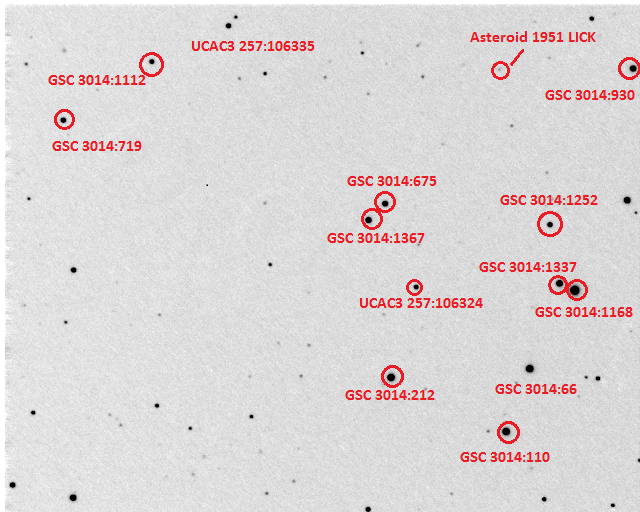
\includegraphics[width=3.4in]{Jul10Series2.png}
\caption{An example of a combined series of images: Series 2 of the observation on July 10 using the Meade 14'' telescope.\label{fig:exampleseries}}
\label{fig_sim}
\end{figure}

\begin{table}[!t]
\centering
\begin{tabular}{|c|c|c|c|c|}
\hline
Date & Telescope & Sync Star & Filter & \# images \\ \hline \hline
July 1 &Meade 14''& \multicolumn{3}{c|}{Omitted due to bad quality}\\ \hline \hline
July 3 & Keck 24''& Arcturis & Clear & 5 \\ \cline{4-5}
 & & & Clear & 5\\ \cline{3-5}
 & & \multicolumn{3}{c|}{Omitted due to bad quality} \\ \hline \hline
July 8 & Meade 14'' &\multicolumn{3}{c|}{Images are of wrong part of sky} \\ \cline{3-5}
 & & Phecda & Clear & 7 \\ \cline{4-5}
 & & & Clear & 7\\ \cline{4-5}
 & & & Clear & 7\\ \hline \hline
July 10 & Meade 14''& Phecda & Clear &7 \\ \cline{4-5}
 & & & Clear & 7\\ \cline{4-5}
 & & & Clear & 7\\ \hline \hline
July 16 & Meade 14''& Phecda & V-filter &5 \\ \cline{4-5}
 & & & Clear & 5\\ \cline{4-5}
 & & & Clear & 5\\ \cline{4-5}
 & & & Clear & 5\\ \cline{4-5}
 & & & Clear & 5\\ \hline \hline
July 19 & Meade 14''& Phecda & Clear &7 \\ \cline{4-5}
 & & & Clear & 7\\ \cline{4-5}
 & & & Clear & 7\\ \cline{4-5}
 & & & Clear & 7\\ \hline \hline
July 25 & Meade 14'' & Phecda & Clear &5 \\ \cline{4-5}
 & & & V-filter & 1\\ \hline
\end{tabular}
\caption{List of image series taken in observations of 1951 Lick in 2011\label{tab:serieslist}}
\end{table}

\subsection{Least-Squares Plate Reduction}
Using a Python program written by the authors that implements least-squares plate reduction (LSPR), 
the equatorial coordinates of the asteroid in each image were calculated.
%LSPR means nothing to people; our goal is not LSPR, but to find asteroid coordinates.
LSPR is a process to find the mapping from the $x$ and $y$ plate coordinates of bright reference stars 
(which are obtained from Maxim DL) to the equatorial coordinates
of each star tabulated in the NOMAD database.
By applying this map to the $x$ and $y$ coordinates of the asteroid, the equatorial coordinates of
the asteroid were obtained.
%Jason: I prefer $x$ and $y$ instead of $xy$. It reads easier to me.
%Pato: I argue $xy$ for the sake of brevity. It also highlights that $xy$ together form a plane, while $x$ and $y$ could just as much use $x$ and $\eta$. Lets settle this before we change anything.
%Jason: I figured it out. I prefer $x$,$y$ rather than $x$ and $y$.

Before LSPR was performed, the effect of altitude on the stars' angle of refraction was accounted for.
%Pato: This is still awkward.
The time of observation given by each image's file information header and the difference between the 
observatory's clock and the US Naval Observatory's clock were used to calculate the local sidereal time.
%Pato: is FITS not something standardized? I think it is. But abstraction is preferred by me, even if the language is very awkward.
This, in turn, was used to convert the equatorial coordinates of each reference star from NOMAD 
into theoretical values for local coordinates of altitude and azimuth.
Using an index of refraction of $n-1=58.2''$ for the atmosphere\footnote{Value as in [2]}, 
the computed altitude of each star was adjusted to account for the resulting offset.
%Pato: Where is this angular estimate from? Cite!
%Pato: Thank you. How is this an assumption?
%David: Good point. Word choice is essential.
The adjusted altitude and azimuth were then converted back to theoretical apparent equatorial coordinates.

To find the mapping between the plate $x$ and $y$ coordinates and the equatorial $\alpha$ and $\delta$ coordinates by LSPR, 
a least-squares linear fit that mapped the $x$ and $y$ plate coordinates of each star to its 
theoretical apparent equatorial coordinates was computed.
Using this mapping, the apparent equatorial coordinates of the center of the image were obtained 
to calculate the standard $\xi$ and $\eta$ coordinates for each reference star.\footnote{See [2]} 
Because the standard coordinates are truly linear functions of the plate coordinates, 
a more accurate least-squares fit was computed that maps the plate coordinates to the standard coordinates.
Using this linear transformation, the $\xi$ and $\eta$ coordinates of the asteroid were obtained, 
from which the apparent $\alpha$ and $\delta$ of the asteroid were calculated.
Finally, the apparent equatorial coordinates were transformed back to equatorial coordinates 
using the same index of refraction of the atmosphere.

To obtain an estimate of the uncertainty of the $\alpha$ and $\delta$ of the asteroid, 
the deviation of the predicted equatorial coordinates of each star 
from the catalogued coordinates were computed assuming two degrees of freedom.
This residual was possibly due to defects in the CCD chip or telescope mirror, 
aberration of starlight, inaccurate tabulations of reference star coordinates, 
or uncertainties in the centroid computations.

\subsection{Orbit Determination using Laplace's Method}
From the measured $\alpha$ and $\delta$ of the asteroid, 
the classical orbital elements of the asteroid were determined. 
Because the asteroid had recently exited from a retrograde loop,
the asteroid's position relative to Earth as a function of time was approximately a straight line,
resulting in small values for the change in velocity
of the unit range vector $\hat{\rho}$, $\frac{d^2\hat{\rho}}{d\tau^2}$.\footnote{$\tau$ is the modified time given by $\tau=kt$, for ordinary time $t$ 
and the Gaussian gravitation constant $k=0.017...$
All time derivatives in this section are with respect to modified time.}
%Pato: The addition of a footnote here makes it looks like we are squaring the derivative. Hence placing the footnote BEHIND the period.
%David: English custom says that footnotes should come before period. But the footnote is confusing
%david: so ideally we should rephrase sentence, but I'll just let it be.
The Gauss-Gibbs method of orbit determination,\footnote{Described in [1]} which is
sensitive to values of $\frac{d^2\hat{\rho}}{d\tau^2}$, produced unrealistic results, and so Laplace's method was used.

Five observations were used to obtain $\frac{d\hat{\rho}}{d\tau}$ and $\frac{d^2\hat{\rho}}{d\tau^2}$ 
for the middle observation.
The five unit equatorial vectors are given by $\hat{\rho}_1$, $\hat{\rho}_2$, $\hat{\rho}_3$, $\hat{\rho}_4$ 
and $\hat{\rho}_5$. 
The middle range vectors give the position of the asteroid on July 8 
and were used to accurately estimate $\frac{d\hat{\rho}}{d\tau}$.
The second derivative of $\hat{\rho}$ at the middle observation was approximated 
using $\hat{\rho}_1$, $\hat{\rho}_3$, and $\hat{\rho}_5$, 
the range vectors of the asteroid on June 27, July 8, and July 25 respectively.\footnote{The June 27 data were obtained by Hyde, Shah, and Zhao} 
%Data is always plural. please don't unedit the grammar.
%Jason: Disagree. Data can be used in both the singular and plural forms, though some prefer it in the plural form only.
%Consider: Much of this data is useless because of its lack of specifics.
%Using "are" instead of "is" makes it ungrammatical because it is talking about "this" data.
%Instead, "Many of these data are useless because of their lack of specifics" is correct.
%However, in this case, we are talking about data from one day AND for one observation. So I suggest 
%that we should use "was" instead of "were". If we said "The June 27, June 29, and June 30 data were
%obtained...." this would be correct. 
%Pato: I looked it up. Both conventions are common. I prefer to stick with what Jason described. David, you have been outvoted.
%Pato: Also, David, remember to sign your discussion comments.
%David: Wow! I did not expect this to be so controversial!
%David: But anyways, data is the plural of the latin noun datum. Although many people use data as singular
%this does not make singular data any more correct. Consider: half the English-speaking world say "different than"
%but that doesn't make it any more correct. More than half the world do not believe in evolution or relativity
%should we use the principle of "truth by democracy" to say the two theories are wrong?
%Usage of plural data shows classical education and respect towards the academic/scientific world, which still prefer plural data.

This time span was chosen to be large enough for the first derivative to change sufficiently.

%Jason: Is this footnote necessary? (about The June 27 data was obtained by the other team)

To compute the first derivative, a second-order Taylor expansion was used:
\begin{eqnarray*}
\hat{\rho}_4&=&\hat{\rho}_3+\hat{\rho}_3' (\tau_4-\tau_3)+\frac{1}{2}\hat{\rho}_3'' (\tau_4-\tau_3)^2\\
\hat{\rho}_2&=&\hat{\rho}_3+\hat{\rho}_3' (\tau_2-\tau_3)+\frac{1}{2}\hat{\rho}_3'' (\tau_2-\tau_3) ^2\\
\end{eqnarray*}
which was solved for $\hat{\rho_3}'$.
The second derivative was calculated similarly but with $\hat{\rho}_1$ and $\hat{\rho}_5$ 
instead of $\hat{\rho}_2$ and $\hat{\rho}_4$.
From $\frac{d\hat{\rho}}{d\tau}$ and $\frac{d^2\hat{\rho}}{d\tau^2}$, 
the standard Laplace method was used to generate the position and velocity vectors of the asteroid.\footnote{See [1]}
This calculation was done using a script written in Python.

From the preliminary position and velocity, 
an ephemeris was generated for the times of each of the observations, 
and the differences from the measured values $\Delta \alpha$ and $\Delta \delta$ were calculated.
The difference between the computed and measured values of $\alpha$ and $\delta$ 
is caused by a small error in the position and velocity according to the equations below:
\begin{eqnarray*}
\Delta \alpha &=& \frac{\partial \alpha}{\partial r_x} \Delta r_x + \frac{\partial \alpha}{\partial r_y} \Delta r_y + \frac{\partial \alpha}{\partial r_z} \Delta r_z + \\& &
\frac{\partial \alpha}{\partial v_x} \Delta v_x + \frac{\partial \alpha}{\partial v_y} \Delta v_y + \frac{\partial \alpha}{\partial v_z} \Delta v_z \\
\Delta \delta &=& \frac{\partial \delta}{\partial r_x} \Delta r_x + \frac{\partial \delta}{\partial r_y} \Delta r_y + \frac{\partial \delta}{\partial r_z} \Delta r_z + \\& &
\frac{\partial \delta}{\partial v_x} \Delta v_x + \frac{\partial \delta}{\partial v_y} \Delta v_y + \frac{\partial \delta}{\partial v_z} \Delta v_z
\end{eqnarray*}
Using six observations of the asteroid, 
least-squares corrections $\Delta r_x$, $\Delta r_y$, $\Delta r_z$, $\Delta v_x$, $\Delta v_y$, and $\Delta v_z$ 
for the position and velocity vectors were found.
Due to inaccurate preliminary vectors, 
these corrected positions and velocities were still not accurate since the differential corrections described above 
only correct for small inaccuracies.
%We had run-on sentence
This process was iterated five times until the computed orbital elements converged,
with the last position and velocity vectors giving new corrected position and velocity vectors according to the 
above procedure. 
As Table~\ref{tab:iterations} shows, 
Laplace's method gives inaccurate results for $\omega$ and $T_P$.
%Pato: I do not see how we can argue improvement of time of perihelion of the HORIZONS value is more wrong than our initial value.
%David: Recall we have periodic motion :) Maybe we should add the period of the asteroid=sqrt(a^3)
%How should we do so? Using the correct value for a, or the incorrect values yielded 
%in each iteration
%Or maybe a better way is to subtract a period from the JPL value.
%Are we fixing this point? Any consensus?
With one iteration of corrections, $\omega$ and $T_P$ are much more accurate, but the other orbital elements
are over-corrected. Each subsequent iteration improves the value of all orbital elements.

\begin{table}[!t]
\centering
\begin{tabular}{|c|c|c|c|c|c|c|}
\hline
No. of Corrections & $a$ [AU]& $e$ & $i$ [$^\circ$] \\ \hline
Laplace's Method &1.376& 0.0699& 39.447 \\ \hline
One iteration &1.342& 0.0576& 38.968 \\ \hline
Two iterations &1.384& 0.0592& 39.078 \\ \hline
Three iterations &1.389& 0.0604& 39.087 \\ \hline
Four iterations &1.389& 0.0604& 39.088 \\ \hline
Five iterations &1.389& 0.0605& 39.088 \\ \hline
HORIZONS Value & 1.390536 & 0.0616082& 39.08962  \\ \hline \hline
No. of Corrections & $\Omega$ [$^\circ$] & $\omega$ [$^\circ$] & $T_P$ [JD]\\ \hline
Laplace's Method & 129.761& 344.711& 2455602.859\\ \hline
One iteration & 131.535& 163.598& 2455298.593\\ \hline
Two iterations & 130.852& 142.718& 2455243.991\\ \hline
Three iterations & 130.777& 140.797& 2455238.203\\ \hline
Four iterations & 130.773& 140.700& 2455237.901\\ \hline
Five iterations & 130.772& 140.695& 2455237.885\\ \hline 
HORIZONS Value & 130.769445 & 140.4418 & 2455835.571 \\ \hline
\end{tabular}
\caption{\label{tab:iterations} 1951 Lick orbital element outputs of Laplace's method, iterations of differential correction, and JPL HORIZONS}
\end{table}

To compute the uncertainties for the orbital elements, 
a normal distribution according to the standard deviation computed from the LSPR 
for the $\alpha$ and $\delta$ of the asteroid was assumed.
A Monte-Carlo method with sample size of five hundred was used to compute the orbital elements using the procedure 
specified above for a set of asteroid coordinates randomly sampled from the Gaussian distribution.
The standard deviation of the computed orbital elements was reported as the uncertainty.

\subsection{Photometry}
On July 16 and July 25, 2011, a V-filter image of the asteroid was taken to measure the V-magnitude of the asteroid.
To determine the apparent magnitude of the asteroid, images were taken with a V-filter in the telescope, 
instead of the clear filter that was used for astrometry.
After taking a series of images with the V-filter, V-magnitudes of surrounding stars were obtained from the NOMAD database.
From the V-magnitudes of the reference stars, MaximDL computed the V-magnitude of the asteroid. See Table~\ref{tab:vmag}.

\begin{table}[!t]
\centering
\scalebox{0.9}{
\begin{tabular}{|c|c|c|}
\hline
Asteroid V-mag & Observation & Sync Star V-mag \\ \hline \hline
16.861 & GSC 2531:1730 & 12.690 \\ \hline
17.122 & GSC 2529:1728 & 12.590 \\ \hline
\end{tabular}
}
\caption{V-magnitude of 1951 Lick \label{tab:vmag}}
\end{table}

\section{Results}

The result of the orbit determination along with the uncertainty are shown in Table~\ref{tab:orbitalelements}.

\begin{table}[!t]
\centering
\scalebox{0.9}{
\begin{tabular}{|c|c|c|}
\hline
$a$ & $e$ & $i$ \\ \hline
$1.3894 \pm 0.0094$ AU & $0.06053 \pm 0.0024$ & $39.089 \pm 0.019 ^{\circ}$ \\ \hline \hline
$\Omega$ & $\omega$ & $T_P$ \\ \hline
$130.7706 \pm 0.1415 ^{\circ}$ & $140.65 \pm 3.71 ^{\circ}$ & $2455237.7 \pm 11.3$ JD \\ \hline
\end{tabular}
}
\caption{Measured orbital elements of 1951 Lick \label{tab:orbitalelements}}
\end{table}

The eccentricity of the orbit of the asteroid is similar to that of Mars with 
$e = 0.093$ \cite{bib:HORIZONS}, 
and the point of perihelion is hard to distinguish from other points, 
so the values for $\omega$ and $T_p$ are more difficult to determine than the other orbital elements.

% Jason: No idea what to do with this picture. It's slightly better than it was before, though
% David: Picture does look unprofessional :)
% Pato: Remove! Exterminate!
%\begin{figure}[!t]
%\centering
%\includegraphics[width=3.5in]{Lick_Orbit2.png}
%\caption{Position of the asteroid relative to the Earth.  The blue loop is that of the Earth's orbit, and the black loop is that of the asteroid.  The positions of the Earth, going clockwise, are those of July 25, July 8, and June 26; the positions of the asteroid, going clockwise, are those of July 25, July 8, and June 26. }
%\label{fig_sim}
%\end{figure}

\begin{table}[!t]
\centering
\scalebox{0.9}{
\begin{tabular}{|c|c|c|c|}
\hline
Quantity & Measurement & HORIZONS Value & Difference \\ \hline
$a$ & $1.3894 \pm 0.0094$ AU & 1.390536 AU & 0.0011 AU \\ \hline
$e$ & $0.06053 \pm 0.0024$ & 0.0616082 & 0.0011 \\ \hline
$i$ & $39.089 \pm 0.019^{\circ}$ & 39.08962$^{\circ}$ & 0.001$^{\circ}$\\ \hline
$\Omega$ & $130.7706 \pm 0.1415 ^{\circ}$ & 130.769445$^{\circ}$ & 0.0012$^{\circ}$\\ \hline
$\omega$ & $140.65 \pm 3.71 ^{\circ}$ &140.4418$^{\circ}$ & 0.21$^{\circ}$\\ \hline
$T_P$ & $2455237.7 \pm 11.3$ JD & 2455835.571 JD & 2.1 JD \\ \hline
\end{tabular}
}
\caption{Measured orbital elements in comparison with JPL HORIZONS orbital elements of 1951 Lick}
\label{tab:HORIZONScomparison}
\end{table}

\begin{table}[!t]
\centering
\scalebox{0.9}{
\begin{tabular}{|c|c|c|c|}
\hline
Date & Observed $\alpha$ & HORIZONS $\alpha$ & Computed $\alpha$ \\
\cline{2-4} & Observed $\delta$ & HORIZONS $\delta$ & Computed $\delta$ \\ \hline \hline
Jul 19 & 12h 24m 7.855s & 12h 24m 3.18s & 12h 24m 7.667s \\
\cline{2-4} & 35$^{\circ}$ 5' 27.33'' & 35$^{\circ}$ 5' 32.0'' & 35$^{\circ}$ 5' 28.89'' \\ \hline
\end{tabular}
}
\caption{Comparison of JPL HORIZONS ephemeris of 1951 Lick and ephemeris from determined orbital elements with observation data\label{tab:observationcomparison}}
\end{table}

\section{Conclusion}
JPL HORIZONS provides values for the orbital elements, which serve as a good comparison to computed results.
The differences between the orbital elements that were determined in the experimental procedure and those given by JPL 
are shown in Table \ref{tab:HORIZONScomparison}.
The discrepancies are significantly less than the statistical errors. 
%There are no discrepancies between
%computed orbital elements and that stored in the JPL HORIZONS database.
% David: Above sentences is redundant since we already pointed out discrepancies
%are less than statistical errors.
%Pato: Agreement is expressed.
An ephemeris for July 19 generated from determined orbital elements was also calculated and compared to observations, 
shown in Table \ref{tab:observationcomparison}.
Since orbital elements are constantly changing due to perturbations from planets,
it is irrelevant to compare ephemerides generaged from
these orbital elements with those generated from
orbital elements from HORIZONS, because the orbital elements of this study 
are fitted to the observations and not the orbit at any precise epoch.
%Jason: I don't like this at all. We first say "Oh, we compared it to HORIZONS". Then "Oh, 
%we can't compare it to HORIZONS and it's a bad comparison".
%Pato: The reaseon we compare it to HORIZONS is to show our data is not junk. But we do need to mention that this was an unfair comparison.
%David: Sorry! I was trying to point out the ephemrides are irrelevant.
However, the accuracy of this orbit determination is of theoretical interest, because 
it demonstrates that accurate orbits can be determined even if Gauss-Gibbs's method diverges
and Laplace's method gives orbital elements that are not within reasonable accuracy.
%due to a non-ideal location of an asteroid with respect to the Earth.
%David: First, the above phrase is a dangling modifier; it is unclear what it describes.
%David: Second, we should be respectful of gauss and gibbs (don't say 'their methods gives nothing reasonable'
%Pato: Good. What about the use of the word 'fails'? Before we said 'gives nonesensical data'. I would suggest 'diverges'. Sound good?

%From the orbital elements, it is clear that there is very low probability the asteroid will hit the Earth in the near future.
%With such a low eccentricity, the asteroid is in a highly circular orbit, minimizing perturbations from other planets.
%Since gravitational acceleration is independent of mass, the stability of the asteroid's orbit is comparable to that of Mars in the short term.
%The successful computation of the orbit of 1951 Lick is an interesting case study, considering the non-ideal location of the asteroid with respect to the Earth.
%Future groups would benefit from our method of orbit determination.

\section*{Acknowledgments}

The authors would like to thank Dr. Michael Faison, Martin Mason, and Mary Masterman, 
Dougal Sutherland, Becky Raph, and Sean Mattingly for their help debugging Python scripts, assistance with observations, and teaching us the methodology used in this project.
The authors are also grateful towards Jeremy Hyde, Pathik Shah, and Ming Zhao for sharing their
data of 1951 Lick.


\begin{thebibliography}{1}
\bibitem{bib:Danby}
Danby, J. M. A. (1962). \emph{Fundamentals of Celestial Mechanics} New York: Macmillan, 1962. 
%J.M.A.~Danby. \emph{Fundamentals of Celestial Mechanics}, 1st~ed.\hskip 1em plus
%  0.5em minus 0.4em\relax New York: Macmillan, 1962.
\bibitem{bib:Tatum}
Tatum, J. B. (2002). \emph{Celestial Mechanics} Obtained from M. Mason in 2011
%J.B.~Tatum. \emph{Celestial Mechanics}, 1st~ed., 2002\hskip 1em plus
%  0.5em minus 0.4em\relax
\bibitem{bib:HORIZONS}
NASA Jet Propulsion Laboratory HORIZONS System. Retrieved from http://ssd.jpl.nasa.gov/?horizons.
\end{thebibliography}

\end{document}